\documentclass[12pt]{article}
\usepackage[utf8]{inputenc}
\usepackage[spanish]{babel}
\usepackage[a4paper, margin=1.5cm]{geometry}
\usepackage{parskip}
\usepackage{array}
\usepackage{booktabs}
\usepackage{hyperref}
\usepackage{graphicx}
\usepackage{float}
\usepackage{makecell}
\usepackage{longtable}
\usepackage{caption}
\captionsetup[table]{labelfont=bf, name=Tabla}

\title{\textbf{Respuesta a la Opinión Escrita de la Solicitud Internacional PCT/IB2025/051638}}
\author{Luis Fernando Vesga Martínez\\Solicitante / Inventor\\\texttt{vesgaluis@edificausa.com}}
\date{\today}

\begin{document}

\maketitle

\section{Respecto a cada sistema referenciado}

\section*{ D1 – US10961682B1 (Williams, 2021)}

\begin{itemize}
    \item \textbf{Uso/Enfoque:} Corrección de foundation heave (levantamiento de cimentaciones) por estabilización térmica y secado del suelo en contacto con los cimientos. El objetivo es reducir la humedad y modificar las propiedades mecánicas del suelo debajo y alrededor de estructuras
    \subsection*{Funcionamiento detallado}

    \begin{enumerate}
        \item \textbf{Inserción de dispositivos de inyección:}
        \begin{itemize}
            \item Se introducen uno o más dispositivos de inyección de aire en el suelo cercano a la cimentación.
            \item Cada dispositivo consiste en un cuerpo alargado (\(\geq\) 3 pies) con una pared lateral perforada.
            \item La relación longitud/diámetro del tubo es \(\geq 100\), optimizando la distribución longitudinal del flujo.
            \item Algunos modelos incluyen hélices en espiral para facilitar la inserción.
        \end{itemize}

        \item \textbf{Preparación del flujo de aire:}
        \begin{itemize}
            \item Un compresor genera aire seco con humedad relativa \(\leq 30\%\) (posiblemente \(\leq 5\%\)).
            \item El aire pasa por un \textit{aftercooler} para enfriamiento preliminar.
            \item Luego es deshumidificado mediante un módulo de secado.
            \item Finalmente, un calentador eleva su temperatura a \(\geq 150^\circ\)F.
        \end{itemize}

        \item \textbf{Inyección al subsuelo:}
        \begin{itemize}
            \item El aire tratado es inyectado al suelo a través de los ductos perforados.
            \item La presión de inyección es de al menos 50~psig.
            \item El aire se dispersa por las perforaciones y reduce el contenido de humedad del suelo circundante.
        \end{itemize}

        \item \textbf{Modificación del suelo:}
        \begin{itemize}
            \item La combinación de aire seco, caliente y presurizado deseca el suelo.
            \item Esto reduce su capacidad de expansión y mejora su resistencia.
            \item El tratamiento se enfoca en zonas localizadas bajo losas o cimentaciones.
        \end{itemize}

        \item \textbf{Inyección de estabilizante (opcional):}
        \begin{itemize}
            \item Tras la fase de aire, puede inyectarse un agente estabilizante líquido por el mismo conducto.
            \item Este se distribuye por las perforaciones hacia el suelo seco.
        \end{itemize}

        \item \textbf{Configuración espacial:}
        \begin{itemize}
            \item Los ductos se insertan a menos de 15~ft de la cimentación.
            \item Pueden estar inclinados entre 25° y 70° desde la horizontal.
        \end{itemize}
    \end{enumerate}
    \item \textbf{Materiales:} Ductos perforados metálicos o de plástico resistente.
    \item \textbf{Flujo de aire:} Inyección con compresor.
    \item \textbf{Componentes:} Calentador (eléctrico), compresor, sensores, sistema de control, válvulas.
    \item \textbf{Proceso:} Calentamiento de aire → compresión → inyección por ductos perforados → interacción con humedad del suelo → secado.
\end{itemize}

\begin{figure}[H]
\centering
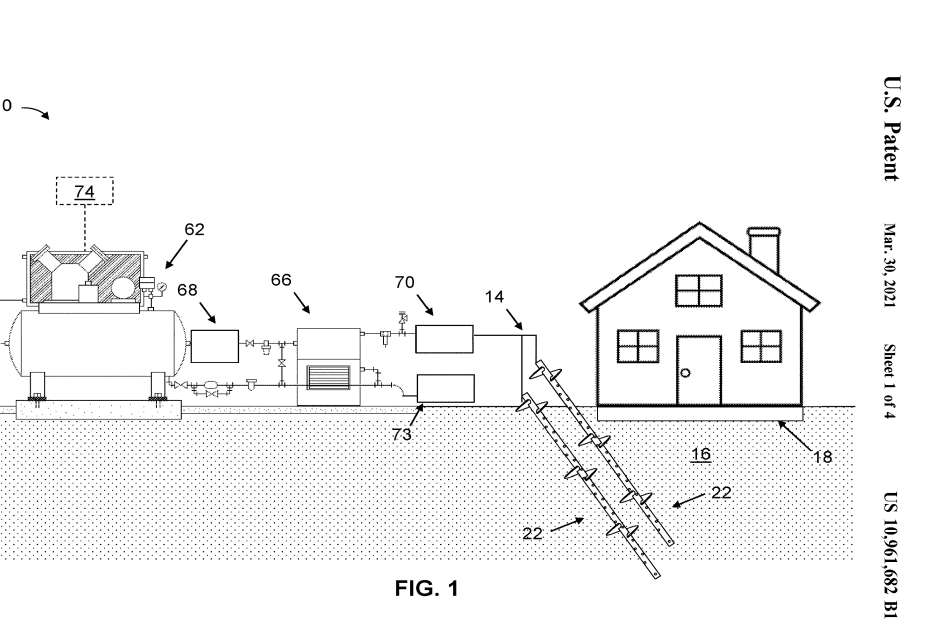
\includegraphics[width=0.6\textwidth]{images/d1_williams.png}
\caption{Esquema ilustrativo del sistema D1.}
\end{figure}

\section*{ D2 – JP2015017399A (Taisei Corp, 2015)}

\begin{itemize}
    \item \textbf{Uso/Enfoque:} Mejora de suelos antes de excavación, especialmente en zonas urbanas sin espacio para secado de material.
    \item \textbf{Funcionamiento:} Inserta tubos horizontales y verticales con calentadores de vapor. El vapor se propaga por perforaciones, calentando el suelo y evaporando el agua. El calor generado por los medios de calefacción se conduce al suelo a través del material de la tubería, y el calor conducido hace que la humedad del suelo se evapore. Esta evaporación puede reducir el contenido de humedad del suelo.
    \item \textbf{Materiales:} Tubos perforados; calentadores de vapor.
    \item \textbf{Flujo de aire:} Vapor inyectado, no se usa aire comprimido.
    \item \textbf{Componentes:} Tubos horizontales/verticales, calentadores de vapor, posible compresor para aire adicional.
    \item \textbf{Proceso:} Inyección de vapor → evaporación del agua
\end{itemize}

\begin{figure}[H]
\centering
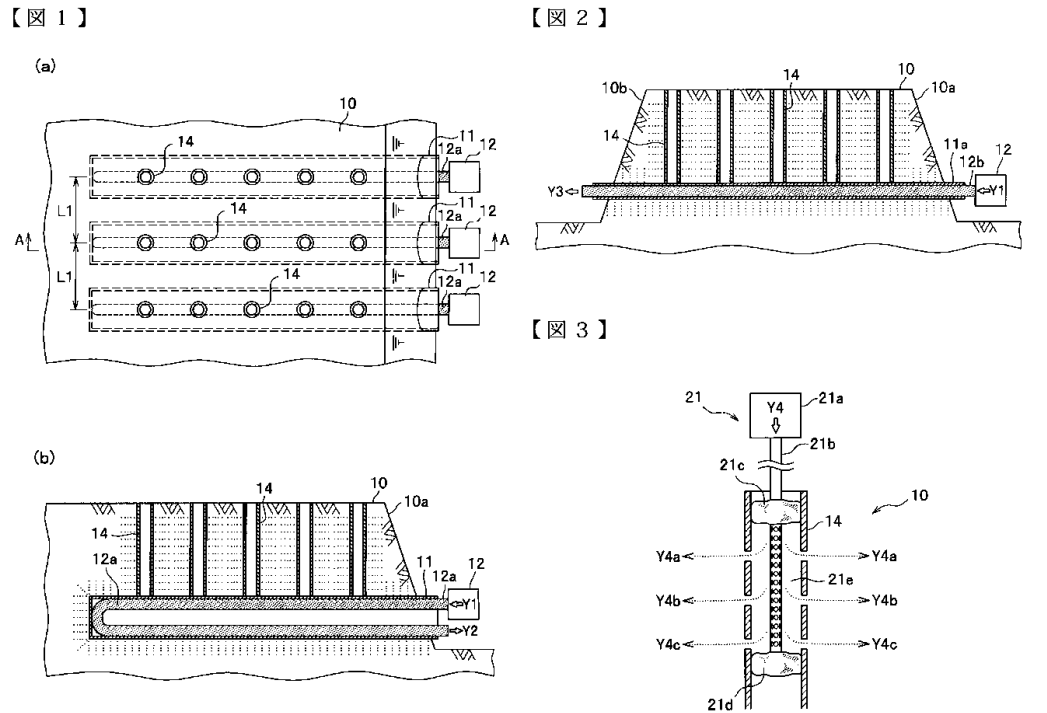
\includegraphics[width=0.7\textwidth]{images/d2_taisei.png}
\caption{Sistema D2 de tratamiento térmico con vapor.}
\end{figure}

\section*{ D3 – US2001002970A1 (Pizzorni et al., 2001)}

\begin{itemize}
    \item \textbf{Uso/Enfoque:} Un dispositivo para tratar el suelo en las proximidades de estructuras enterradas, comprende una pluralidad de sondas que se introducen en el subsuelo y están conectadas a una unidad de control provista de un dispositivo generador de aire para generar, dentro del suelo, un flujo de aire seco. Las sondas están dispuestas de forma que el aire generado circule por todas las superficies de las estructuras enterradas.

    \item \textbf{Funcionamiento:} Se entierran varias sondas (probes) en el subsuelo alrededor de las estructuras. Estas están conectadas a una unidad central de control que inyecta aire seco (previamente calentado) a través de algunas sondas (conjunto de inyección), mientras otras sondas actúan como extractoras, generando un flujo controlado de aire que rodea las superficies de las estructuras enterradas.El sistema incluye sensores para detectar parámetros del flujo y ajustar su operación.

    \item \textbf{Materiales:} Pozos, ductos, resistencias térmicas.
    \item \textbf{Flujo de aire:} Inyección de aire caliente + posible succión.
    \item \textbf{Componentes:} Calentadores, compresores, sensores, ventiladores.
    \item \textbf{Proceso:} Calentamiento → inyección → evaporación → posible captura con vacío.
\end{itemize}

\begin{figure}[H]
\centering
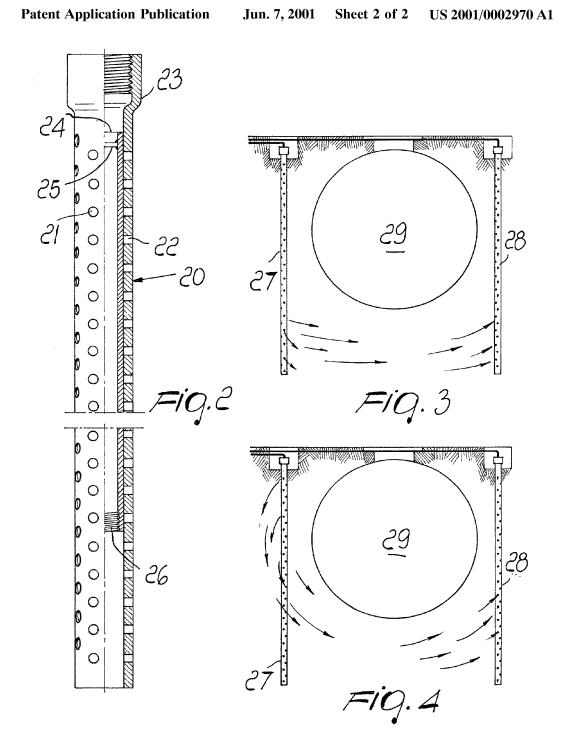
\includegraphics[width=0.4\textwidth]{images/d3_pizzorni.png}
\caption{Sistema D3 de remediación térmica con aire caliente.}
\end{figure}

\section*{ D4 – ES2895271A1 (Amador, 2022)}

\begin{itemize}
    \item \textbf{Uso/Enfoque:} Secado de suelo en zonas agrícolas y de construcción.
    \item \textbf{Funcionamiento:} Tubo interior de PVC perforado se instala en el suelo, envuelto con malla. Se introduce aire mediante un ventilador/motor, generando flujo por el tubo perforado, haciendo que haya un flujo de aire facilitando la expulsion de la humedad a la atmosfera, mediante el intercambio de aire entre los dos medios, subsuelo-atmosfera, de forma que el aire con gran presencia de agua es sustituido por el existente en el exterior (atmosfera) con menor concentracion-presencia de humedad.
    \item \textbf{Materiales:} PVC, malla exterior.
    \item \textbf{Flujo de aire:} Inyección con ventilador.
    \item \textbf{Componentes:} Ventilador, tubos interiores/exteriores, sistema de soporte.
    \item \textbf{Proceso:} Aire impulsado → circulación por perforaciones → secado del suelo.
\end{itemize}

\begin{figure}[H]
\centering
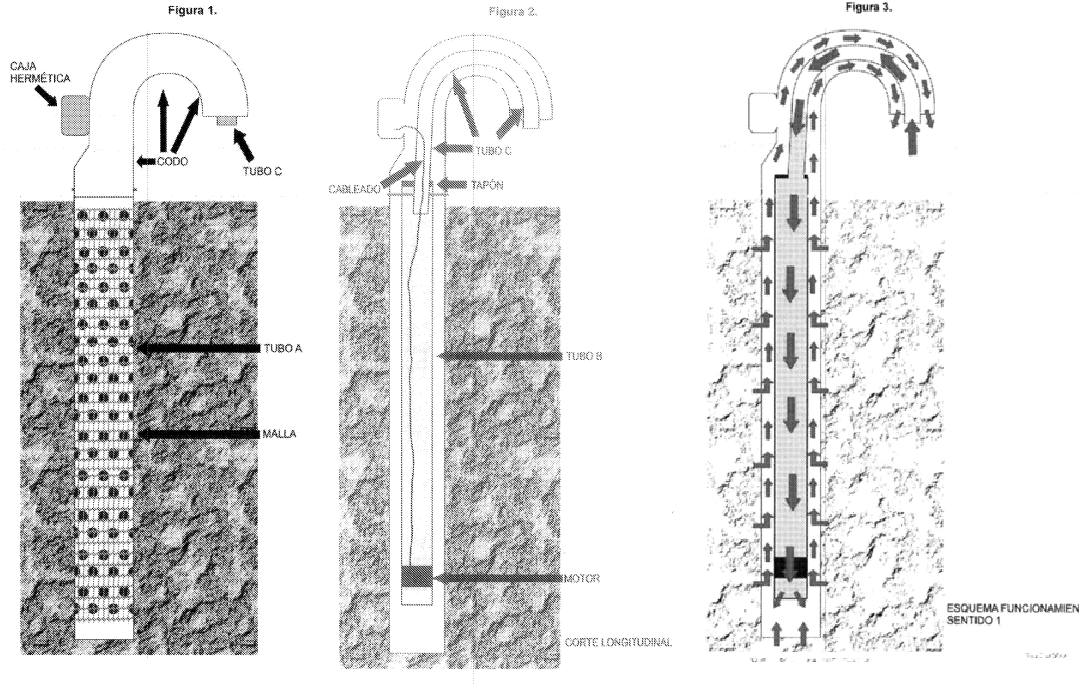
\includegraphics[width=0.7\textwidth]{images/d4_amador.png}
\caption{Esquema del sistema D4 con ventilación agrícola.}
\end{figure}

\section*{ D5 – SU1351999A1 (URSS, 1987)}

\begin{itemize}
    \item \textbf{Uso/Enfoque:} Reforzamiento térmico de suelos de subsidencia.
    \item \textbf{Funcionamiento:} Se perfora un pozo central (well 1), equipado con válvulas, boquillas y conexión a un tanque de combustible y un compresor. Se inyectan pulsos de gases calientes generados por combustión, que elevan la temperatura del suelo y provocan la expulsión de agua hacia el entorno. Luego se perforan varios pozos satélites (boreholes 6) alrededor del pozo principal, desde los cuales se extrae el agua acumulada mediante bombeo. Posteriormente, se inyecta aire en el pozo principal para continuar el calentamiento y consolidación del suelo, repitiendo el ciclo hasta alcanzar una temperatura estable que garantice la eliminación de la subsidencia.
    \item \textbf{Materiales:} Pozos, tuberías, termopares.
    \item \textbf{Flujo de aire:} Inyección de gases calientes + aire.
    \item \textbf{Componentes:} Compresor, bomba, válvulas, sensores.
    \item \textbf{Proceso:} Inyección de gases → redistribución → extracción de agua → monitoreo térmico.
\end{itemize}

\begin{figure}[H]
\centering
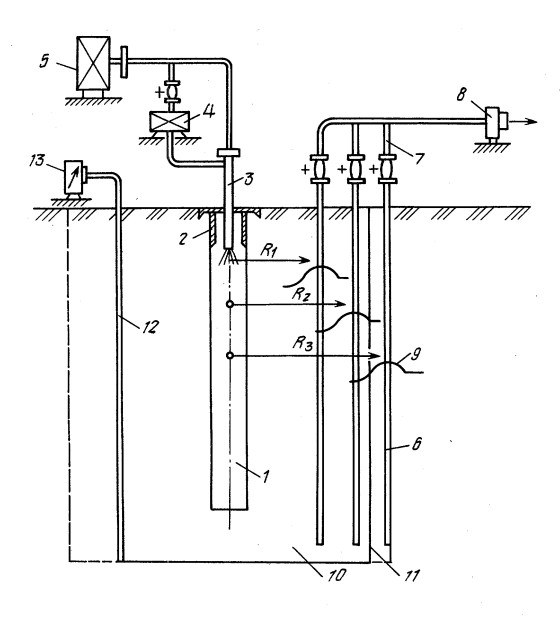
\includegraphics[width=0.5\textwidth]{images/d5_urss.png}
\caption{Sistema D5 para tratamiento térmico por pulsos.}
\end{figure}

\section*{ D6 – SU1491959A1 (URSS, 1989)}

\begin{itemize}
    \item \textbf{Uso/Enfoque:} Consolidación térmica de suelos colapsables.
    \item \textbf{Funcionamiento:} Se forman los pozos principales 1 y auxiliares 2, se sella la boca de cada pozo 1,2 con válvulas, mientras se inyecta aire atmosférico en el pozo principal, se comprueba que no hayan fugas en el sistema. La humedad se condensa en zonas frías del suelo y luego se extrae con aire.
    \item \textbf{Materiales:} Pozos, válvulas, tuberías.
    \item \textbf{Flujo de aire:} Inyección atmosférica + vacío.
    \item \textbf{Componentes:} Compresor, bomba de vacío, sensores.
    \item \textbf{Proceso:} Vacío → inyección → condensación → secado térmico.
\end{itemize}

\begin{figure}[H]
\centering
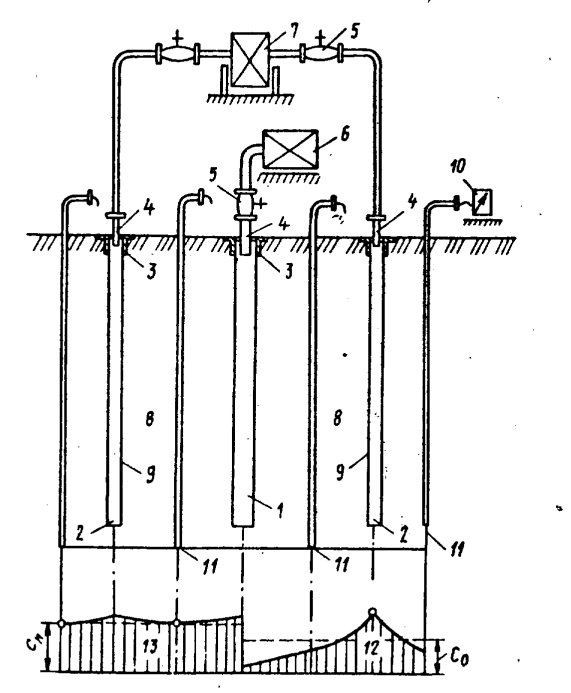
\includegraphics[width=0.4\textwidth]{images/d6_urss.png}
\caption{Sistema D6 de consolidación térmica por vacío.}
\end{figure}

\section*{D7 – EP0597154A1 (Sperry-Sun Drilling Services, 1994)}

\begin{itemize}
    \item \textbf{Uso / Enfoque:} Descontaminación in-situ de formaciones terrestres contaminadas, especialmente por compuestos orgánicos volátiles o hidrocarburos. El objetivo principal es la \textit{remediación ambiental} mediante tratamiento térmico subterráneo.

    \item \textbf{Funcionamiento:} Se perfora un pozo donde se introduce una fuente de combustible (gas o líquido) en el fondo. Aire o gas precalentado a altas temperaturas  se inyecta en el pozo, donde se enciende al contactar con el combustible. La combustión eleva aún más la temperatura , generando gases calientes que se expanden hacia el suelo contaminado. Esto volatiliza u oxida los contaminantes, que son luego extraídos hacia la superficie.

    \item \textbf{Materiales:} Pozos perforados, líneas de inyección de aire y combustible, recubrimientos térmicos resistentes, sensores de temperatura y presión.

    \item \textbf{Flujo de aire / agua:} 
    \begin{itemize}
        \item Inyección de aire/gas presurizado (alta temperatura).
        \item Gases calientes se expanden desde el pozo hacia la formación.
    \end{itemize}

    \item \textbf{Proceso:} Preparación del pozo → inyección de gas caliente + combustible → ignición subterránea → combustión intensificada → gases calientes se expanden → volatilización u oxidación de contaminantes → extracción de vapores en superficie.
\end{itemize}

\begin{figure}[H]
\centering
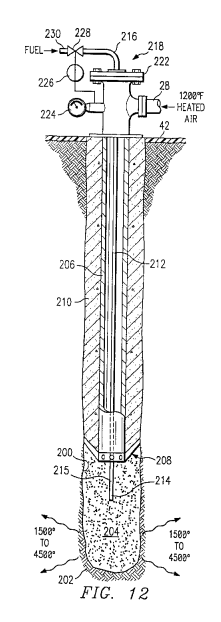
\includegraphics[width=0.2\textwidth]{images/d7_sperry_sun.png}
\caption{Esquema del sistema D7 de descontaminación térmica in-situ.}
\end{figure}

\section*{ D8 – JP2014084559A (Maeda, 2014)}

\begin{itemize}
    \item \textbf{Uso/Enfoque:} Mejora de subrasantes por evaporación al vacío sin sellado superficial.
    \item \textbf{Funcionamiento:} Se instalan pozos conectados a bombas de vacío y compresores. Se genera zona insaturada y se inyecta aire para atrapar burbujas en el suelo.
    \item \textbf{Materiales:} Pozos, filtros, mangueras, tuberías.
    \item \textbf{Flujo de aire:} Succión + inyección.
    \item \textbf{Componentes:} Bomba de vacío, compresor, blower, válvulas, filtros.
    \item \textbf{Proceso:} Succión de aire/agua → formación de zona insaturada entre tuberías → inyección de aire para generar flujo negativo → atrapamiento de burbujas → restauración del nivel freático.
\end{itemize}

\begin{figure}[H]
\centering
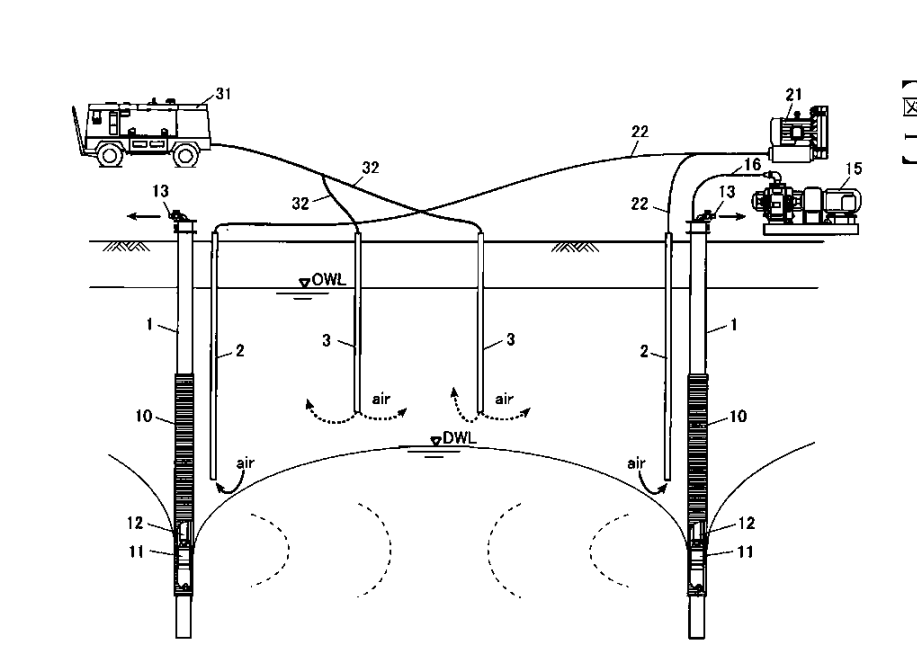
\includegraphics[width=0.7\textwidth]{images/d8_maeda.png}
\caption{Esquema del sistema D8 de evaporación al vacío.}
\end{figure}


\section*{2. Respecto a la falta de novedad}

Se indica que las reivindicaciones 1–3, 5, 7, 10, 14–16 y 19 no son novedosas en vista de los documentos D1, D2 y D3. No obstante, considero que:

\begin{itemize}
    \item El sistema descrito en nuestra solicitud, si bien comparte algunos elementos estructurales con los documentos citados, presenta una \textbf{configuración específica y combinada} de elementos (generador de aire de baja humedad, conducto perforado envuelto en geotextil, bomba para extraer agua en caso de nivel freático, cámara de secado, medición de temperatura y humedad relativa, entre otros, succión de agua por disminución de presión de poros en el suelo) que no se revela de manera anticipada ni explícita en su conjunto en los documentos D1 a D8.
    \item \begin{figure}[h]
    \centering
    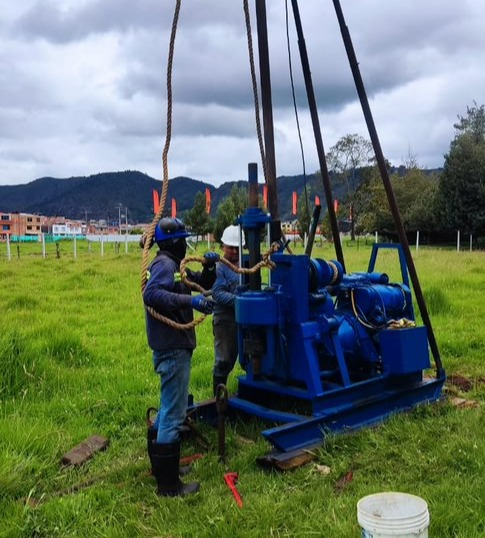
\includegraphics[width=0.4\textwidth]{images/perforacion.JPG}
    \caption{Perforación para la instalación del sistema.}
    \label{fig:perforacion}
    \end{figure}

    \item Además, la \textbf{orientación y propósito de la invención} Se centran en lograr la estabilización del suelo por medio de un secado homogéneo, económico y controlado de suelos finos en condiciones particulares, permitiendo un aumento en el esfuerzo efectivo y por tanto un aumento en la estabilidad general del terreno. Este objetivo no se contempla en los enfoques técnicos ni en las configuraciones descritas por los documentos D1 a D8.
\end{itemize}

\subsection*{Descripción del sistema}

Nuestro sistema contempla la operación en condiciones bajo el nivel freático, incorporando una bomba de extracción que permite manejar flujos de agua que puedan ingresar a través de la perforación. Este componente hidráulico no se menciona en los documentos D1 a D8 y permite ampliar la aplicabilidad del sistema a condiciones de alta saturación, lo que representa una ventaja técnica no anticipada.
\begin{figure}[h]
\centering
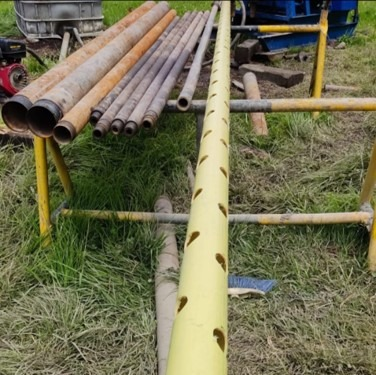
\includegraphics[width=0.4\textwidth]{images/tubo_perforado.jpg}
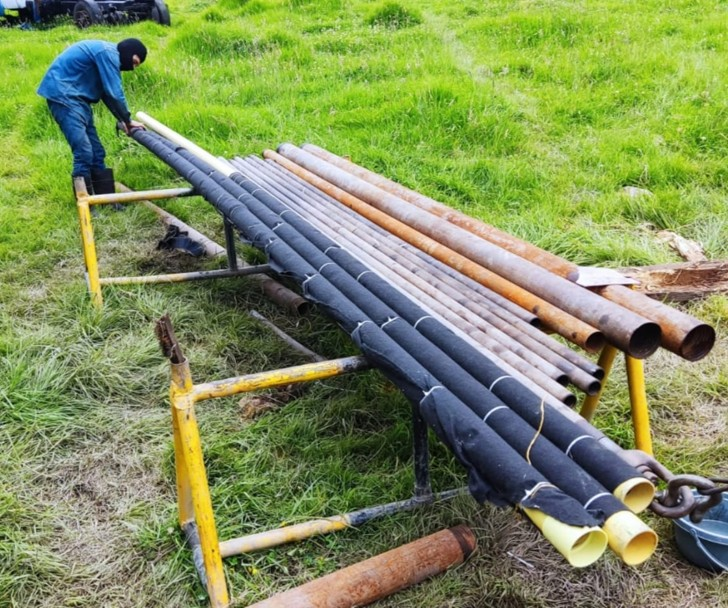
\includegraphics[width=0.475\textwidth]{images/tubo_geotextil.jpg}
\caption{Tubería perforada recubierta de geotextil.}
\label{fig:tubo_geotextil}
\end{figure}


Nuestro sistema contempla la ejecución de perforaciones verticales hasta alcanzar profundidades específicas, principalmente en suelos finos, utilizando maquinaria de tipo rotación y percusión, para generar un conducto profundo (ver Figura \ref{fig:perforacion}). En estas perforaciones se introduce un tubo perforado recubierto de geotextil (ver Figura \ref{fig:tubo_geotextil}), el cual tiene dos funciones principales, primero evitar el flujo de materiales finos hacia dentro del tubo, y segundo generar una separación que permite la transferencia agua desde el suelo hacia el interior de la tuberia y la transferencia del aire desde el tubo hacia el suelo, lo cual también lo diferencia de otras configuraciones (ver Figura \ref{fig:geotextile}).

\begin{figure}[h]
\centering
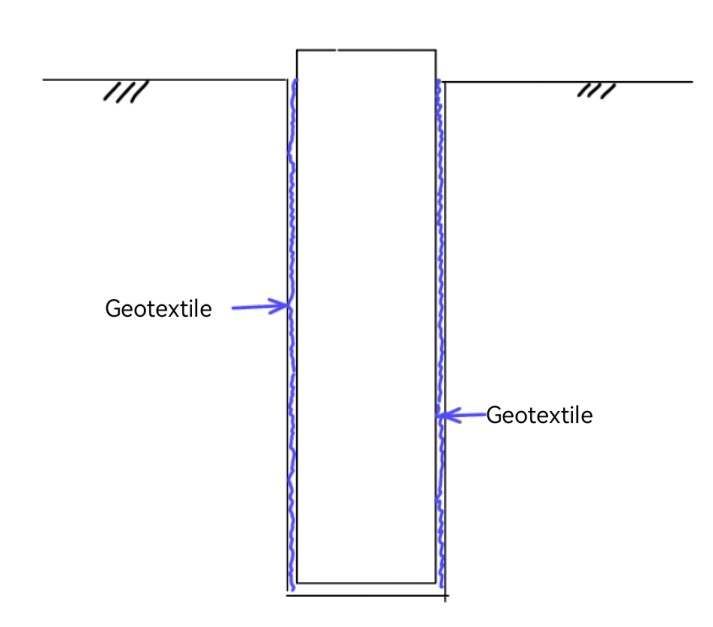
\includegraphics[width=0.4\textwidth]{images/geotextile.jpg}
\caption{Esquema del tubo perforado recubierto de geotextil en la perforación.}
\label{fig:geotextile}
\end{figure}

El sistema opera a presión atmosférica abierta, lo cual representa una diferencia funcional sustancial respecto a otros sistemas que funcionan generando vacío o inyectando un flujo a presión. El aire seco con humedades relativas bajas se introduce en el tubo perforado, generando un flujo de forma ascendente desde el fondo de la perforacion, haciendo que el aire se seco se sature al alcanzar la temperatura de rocio necesaria para que haya condensación del agua en el interior del tubo. Esto genera que el agua presente en los poros del suelo se extraiga de manera controlada y generando un fenomeno de succion que depende en gran medida del contenido de humedad del suelo En ningún momento se busca incrementar la presión de poros del suelo; por el contrario, se reduce la humedad relativa del aire en el interior del tubo perforado, permitiendo así una extracción controlada del agua por gradiente de presión de vapor y un fenómeno de succión que permite la extracción del agua sin incrementar la presión intersticial. Esto es crítico para evitar riesgos de licuación o colapso del terreno.




\section*{3. Pruebas realizadas}

\begin{table}[H]
\centering
\caption{Parámetros de la prueba en Chía}
\begin{tabular}{ll}
\toprule
\textbf{Parámetro} & \textbf{Valor} \\
\midrule
Número de perforaciones & 1 \\
Profundidad total       & 12 m \\
Diámetro                & 3 in \\
\bottomrule
\end{tabular}
\end{table}


\section*{5. Elementos diferenciadores sustanciales}

\begin{enumerate}
    \item \textit{Envoltorio técnico poroso alrededor del ducto perforado}, como geotextil, no presente en D1, D2 ni D4 con la misma finalidad funcional.
    \item \textit{Recirculación de aire post-drenaje en cámara de secado}, ausente en D1 y D2.
    \item \textit{Medición distribuida de temperatura y HR en zonas interiores y exteriores}, superando a D1 y D5.
    \item \textit{Uso combinado de succión (agua) e inyección de aire seco o templado}, sin precedentes en D2 o D8.
    \item \textit{Modificación física del suelo sin remoción previa ni sellado superficial}, a diferencia de D8.
    \item \textit{Modularidad del sistema: configuraciones horizontales, verticales o inclinadas}, frente a esquemas rígidos de D2 y D3.
    \item \textit{Sin uso de vapor o gases calientes}, reduciendo riesgos energéticos u operacionales respecto a D2, D5 y D6.
\end{enumerate}

\section*{6. Conclusión}

Solicito se reconsidere la evaluación de novedad y actividad inventiva a la luz de los argumentos presentados, resaltando el enfoque integral y técnico de la invención, su aplicabilidad específica y la solución novedosa a una problemática real en ingeniería de suelos.

\vspace{2em}
\noindent
\textbf{Luis Fernando Vesga Martínez} \\
Solicitante / Inventor \\
Bogotá, Colombia \\
\texttt{vesgaluis@edificausa.com}

\end{document}
